% =====================================================================
% A Residual Census of Unidentified Chandra Sources in Omega Centauri
% Tim Swanson -- The Omega Centauri Society / Post Oak Labs
% Build: pdflatex census-paper && bibtex census-paper && pdflatex x2
%
% Computation of record: paper/g/analysis/run_g.py (seed 20260814)
%   -> analysis/results_omega_cen.json, analysis/results_control_47tuc.json
%   -> analysis/ANALYSIS_REPORT.md   (WU OCS-G-ANALYSIS-1)
% Data provenance: paper/g/data/DATA_REPORT.md + xray_census.json,
%   msp_counterparts.json, control_47tuc.json (WUs OCS-G-DATA-1/2)
% Number-provenance map: paper/g/DRAFT_EDITLOG.md
% =====================================================================
\documentclass[11pt]{article}

\usepackage[margin=1.1in]{geometry}
\usepackage{newtxtext,newtxmath}
\usepackage[round,authoryear]{natbib}
\usepackage{graphicx}
\usepackage{booktabs}
\usepackage{amsmath}
\usepackage{tikz}
\usepackage{pgfplots}
\pgfplotsset{compat=1.17}
\usepgfplotslibrary{fillbetween}
\usepackage[font=small,labelfont=bf]{caption}
\usepackage{microtype}
\usepackage[colorlinks=true,linkcolor=blue!50!black,citecolor=blue!50!black,urlcolor=blue!50!black]{hyperref}
\usepackage{xcolor}

\newcommand{\msun}{\ensuremath{M_\odot}}
\newcommand{\ocen}{$\omega$~Cen}
\newcommand{\as}{\ensuremath{^{\prime\prime}}}
\newcommand{\pchance}{\ensuremath{P_{\mathrm{chance}}}}
\newcommand{\specbox}[1]{\par\smallskip\noindent\fbox{\parbox{0.97\linewidth}{\small\textbf{Epistemic status:} #1}}\smallskip\par}

\title{\textbf{A Residual Census of Unidentified X-ray Sources in Omega Centauri after the Modern Pulsar Catalogue}}
\author{Tim Swanson\\[2pt]
\small The Omega Centauri Society / Post Oak Labs\\
\small \texttt{tim@postoaklabs.com}}
\date{August 2026 \\[4pt] \small v1.1 (last revised 2026-08-20) --- eighth paper of the set (Paper G); companion to the Macro\\ \small Transcension Hypothesis (Paper A), the inward-migration review (Paper B), the Omega Centauri campaign\\ \small (Paper C), the migration economics (Paper D), the engineered-IMBH systems paper (Paper E), the joint\\ \small accretion bound (Paper F), and the mass-tension paper (Paper H); prepared for omegacentauri.me}

\begin{document}
\maketitle

\begin{abstract}
\noindent
The deepest Chandra catalogue of Omega Centauri \citep{Henleywillis2018} lists 233 X-ray sources, 188 of them without an optical identification, and notes that more than 30 of the unidentified sources carry luminosities and X-ray colours resembling millisecond pulsars (MSPs) in other clusters. That catalogue was published when no radio MSP was known in the cluster. Nineteen are known now \citep{ColomiBernadich2026}, and the catalogue has never been cross-matched against them as a set. We supply that cross-match and the residual census it leaves behind, running the identical pipeline on 47~Tucanae first as a control. The control recovers 18 of 21 known MSP X-ray counterparts at the 95\,per~cent match radius, and the three it misses are the three rows the source catalogue itself flags as deviating beyond that radius \citep{Bhattacharya2017}, so the pipeline reproduces the control's own flag set rather than an independent error budget. In \ocen{} the Chandra astrometric frame carries a measured $+0.42\as$ declination offset relative to the radio frame; registering it takes tier-1 matches from three of eight to five of eight and, with the new timing positions, tightens two published associations from $2.65\as$ and $2.42\as$ to $0.07\as$ and $0.01\as$. All five registered associations sit between $0.01\as$ and $0.35\as$ with per-source chance-coincidence probabilities below $2.3\times10^{-3}$ under each of three independent estimators, reported separately and never combined. One published association is discrepant: the timing position of MSP~H sits $1.81\as$ from source 14c after registration, in the opposite declination sense to the other five anchors, against the $0.73\as$ offset quoted for the same pulsar in \citet{ZhaoHeinke2023}. We record that as a data-quality finding rather than reconciling it. This is a positional and colour census; variability is deferred and addressed only in the back matter. After subtracting a log~$N$--log~$S$ background expectation of 146.9 (92.4--215.5) sources from the 159 unidentified sources inside a $480\as$ aperture, the residual is 12.1 ($-56.5$, $+66.6$), consistent with zero and dominated by the background bracket. Between 39 and 53 unidentified sources fall inside a colour-flux region defined by this cluster's own confirmed counterparts, a quantity that is not interchangeable with the catalogue's own ``more than 30''. The two published population predictions disagree, predicted totals of 324 and 6 pulsars (a factor of 54), which against 19 known imply 176.6 and zero X-ray-detectable undiscovered pulsars \citep{Yin2024}. We bound that disagreement against the residual without adjudicating it. The residual is an input to future identification work and is not a detection of anything.
\end{abstract}

\bigskip
\noindent\textbf{Keywords:} globular clusters: individual: NGC 5139 (Omega Centauri); X-rays: binaries; pulsars: general; catalogues; methods: statistical

\newpage
\tableofcontents
\newpage

\section{Introduction}
\label{sec:intro}

\citet{Henleywillis2018} identify 233 X-ray sources in a 222\,ks Chandra ACIS-I exposure of Omega Centauri (two epochs, 173.7 and 48.5\,ks, per the source paper's own description; distinct from the deeper 290.9\,ks, four-pointing reduction \citet{ZhaoHeinke2023} use for their own X-ray analysis of the same field), 95 of them new, reaching a limiting unabsorbed flux in the core of $f_X(0.5\text{--}6.0\,\mathrm{keV}) \simeq 3\times10^{-16}\,\mathrm{erg\,s^{-1}\,cm^{-2}}$. Forty-five of those sources carry a likely optical identification. The remaining 188 do not. The catalogue's own summary of that unidentified population is the sentence this paper takes as its starting point: no radio millisecond pulsar was then known in the cluster, and more than 30 unidentified sources had luminosities and X-ray colours like those of MSPs found elsewhere.

The situation has since inverted. MeerKAT found 13 pulsars in the cluster \citep{Chen2023}, and the TRAPUM and Parkes programme now reports a timing set of 19 \citep{ColomiBernadich2026}. \citet{ZhaoHeinke2023} identified X-ray counterparts for 11 of the 18 MSPs known at the time of their work, nine of them new. The catalogue of unidentified X-ray sources and the catalogue of radio pulsars therefore both exist, and neither has been confronted with the other as a set. The confrontations that have been made are partial and local. \citet{ColomiBernadich2026} note a marginal positional consistency between pulsar G and Chandra source 24f through an ATCA position and identify 24f as G's counterpart in their conclusions, and they note pulsar L as positionally consistent at roughly $3\sigma$ with source 32d. Those two statements are the prior art this paper extends, and they are credited as such.

Doing the cross-match systematically yields a set of associations with stated false-association rates, which the partial treatments do not carry, and a residual population of unidentified sources that survives every known counterpart class and the expected extragalactic background. The residual is the object of interest and the survey's target list. A count of unidentified sources in excess of a background model is a statement about the completeness of identification work in a crowded, unevenly exposed field, and it constrains nothing on its own.

The referee-facing risks in a paper of this kind are well known and each is addressed mechanically rather than rhetorically. Every probe carries a chance-coincidence probability from three independent estimators (Section~\ref{sec:method-chance}), since positional cross-matching in a crowded core is uninterpretable without a false-association calibration, and membership enters as a probability under stated external normalisations rather than as a binary label (Section~\ref{sec:method-membership}), since colour-box classification without membership priors has no content. The background enters through a published log~$N$--log~$S$ relation with its parameter uncertainties propagated as a bracket (Section~\ref{sec:method-agn}) because extragalactic contamination dominates a field this deep; fluxes near the detection limit are biased high, stated as a direction of error rather than corrected; and the whole pipeline is validated on a control cluster before it is allowed to produce a number for \ocen{} (Section~\ref{sec:control}).

Section~\ref{sec:data} fixes the catalogues and their provenance. Section~\ref{sec:method} gives the cross-match, the three chance estimators, the frame registration, the membership treatment, and the background accounting. Section~\ref{sec:control} reports the control validation. Section~\ref{sec:results} gives the \ocen{} cross-match, the discrepant association, and the residual census. Section~\ref{sec:tension} carries the population-model disagreement. Section~\ref{sec:discussion} states what would identify the residual. Appendix~\ref{app:caveats} collects the caveats as a checklist.

\specbox{Everything in Sections~\ref{sec:data}--\ref{sec:tension} is a count, a measured separation, or an expectation from a cited external relation. No detection is claimed anywhere in this paper, and the residual population is presented as an input to future identification work.}

\section{Data}
\label{sec:data}

\subsection{The X-ray catalogue}
\label{sec:data-xray}

The source catalogue is \citet{Henleywillis2018}, obtained as the machine-readable table from VizieR (\texttt{J/MNRAS/479/2834}) and parsed by byte-column specification rather than transcribed. The parse reproduces the paper's own abstract totals exactly: 233 sources, 95 new, 45 with a likely optical identification. Each source carries a position, a 95\,per~cent confidence error radius, an offset from the \citet{AndersonvanderMarel2010} cluster centre in units of the $155\as$ core radius, detected and exposure-corrected counts in the medium (0.5--4.5\,keV), soft (0.5--1.5\,keV) and hard (1.5--6.0\,keV) bands, unabsorbed fluxes, the soft-to-hard colour $\log(\mathrm{soft}/\mathrm{hard})$, and an optical identification field whose null value defines the unidentified population.

\subsection{The pulsar positions}
\label{sec:data-psr}

Pulsar positions come from \citet{ColomiBernadich2026} and are sorted into precision tiers before any matching is attempted, because a single match radius applied across a set with heterogeneous astrometry is the standard way to manufacture associations.

\begin{description}
\item[Tier 1, eight pulsars (A, B, C, D, E, G, H, K).] Timing-derived positions at milliarcsecond scale. The radio positional uncertainty is set to zero, so the match radius is carried entirely by the X-ray error circle.
\item[Tier 2, five pulsars (I, L, N, Q, S).] Positions from orbital solutions with no formal uncertainty quoted, plus the SeeKAT localisation of S at $\pm1.5\as$. For the four without a stated error we adopt one unit in the last quoted digit as the uncertainty. That rule is ours and not the source paper's, and it is why tier~2 is reported separately and not merged into a headline count.
\item[Null, six pulsars (F, J, M, O, P, R).] No position in \citet{ColomiBernadich2026}, attributed there to \citet{Chen2023}. These six are absent from the cross-match entirely. Recovering their positions from the discovery paper would extend the probe set by six probes and is the cheapest improvement available to this analysis.
\end{description}

\subsection{The published counterparts}
\label{sec:data-counterparts}

\citet{ZhaoHeinke2023} report X-ray counterparts for 11 of the 18 MSPs known at the time, of which seven carry a cross-reference to a \citet{Henleywillis2018} identifier: B$\to$13d, C$\to$23g, E$\to$11f, G$\to$24f, H$\to$14c, K$\to$21d, L$\to$32d. Their tables were read from the published PDF page by page and the positions and luminosities re-verified against that read. Five of the eleven rows required correction of the luminosity uncertainty from a symmetric placeholder to the asymmetric interval the source paper quotes; central values were unaffected. We do not re-derive the luminosity-companion-mass correlation of that paper, which is their result and not ours.

\subsection{Source 24f as a classification-supersession case}
\label{sec:data-24f}

\citet{Henleywillis2018} classify source 24f as \texttt{RGB/SGB-a}, an anomalous red-giant-branch or sub-subgiant candidate. Later radio work identifies the same source as the X-ray counterpart of MSP~G \citep{ZhaoHeinke2023,ColomiBernadich2026}, and after frame registration the timing position sits $0.071\as$ from it (Section~\ref{sec:results-match}). This is the one class assignment in the catalogue known to have been superseded by later radio work.

We carry 24f under its published class in every count reported in this paper and describe the supersession separately. Silently reclassifying one source because a later result is known would make the classification census a mixture of two epochs of knowledge, and the residual would then depend on which supersessions happened to be noticed. Reporting the case explicitly costs one paragraph and keeps the census reproducible from the published tables alone. It also sets the scale of the effect: one source in 233, in a catalogue whose identification work was done before any cluster MSP was known.

\subsection{The control catalogue}
\label{sec:data-control}

The control is 47~Tucanae, from \citet{Bhattacharya2017}, vendored from VizieR (\texttt{J/MNRAS/472/3706}) under the same byte-parse discipline. The record counts reproduce the source exactly: 370 sources within the half-mass radius, a 21-row MSP X-ray position-deviation table, and a 5-row table of new optical counterparts.

One trap in that paper deserves flagging because it would corrupt a control comparison built on the title alone. The title phrase ``five new X-ray counterparts to millisecond radio pulsars'' does not describe five new MSP counterparts. The five new optical counterparts of the paper's table~5 are chromospherically active BY~Dra and W~UMa variable stars. The five MSPs named in the abstract are five pulsars given new spectral extractions. The MSP counterpart truth set for a control comparison is the 21-row deviation table, which covers effectively all known 47~Tuc MSPs, and that is the table used here.

Two asymmetries between control and target are relevant to the design and are not pipeline artifacts. The control's MSP identification is close to complete, 21 counterparts against roughly 23 known pulsars, where \ocen{} sits at 11 counterparts among 18 to 19 known. And the luminosity bands differ, 0.5--6\,keV for the control against 0.5--10\,keV for \ocen, so no cross-cluster luminosity comparison is made anywhere in this paper.

\section{Methods}
\label{sec:method}

\subsection{Tiered cross-match}
\label{sec:method-match}

For each pulsar probe $i$ and X-ray source $j$ the match radius is
\begin{equation}
r_{ij} = \sqrt{\sigma_{\mathrm{radio},i}^{2} + \epsilon_{95,j}^{2}},
\end{equation}
where $\epsilon_{95,j}$ is the catalogue's tabulated 95\,per~cent error circle radius and $\sigma_{\mathrm{radio},i}$ is the radio positional uncertainty of the tier. A probe matches the nearest source inside its radius. Tiers are matched and reported separately throughout. The same code path, with no parameter changes, runs on the control.

\subsection{Three chance-coincidence estimators}
\label{sec:method-chance}

Every probe carries three independent estimates of the probability that its match is a coincidence, each computed with $2\times10^{4}$ trials at a fixed seed.

\begin{description}
\item[Azimuthal rotation.] The probe position is rotated about the cluster centre by a uniform random angle, preserving its cluster-centric radius and therefore the local surface density, and the match is re-attempted.
\item[Catalogue offset.] The source catalogue is displaced by a random vector large compared with the match radius and small compared with the field, and the match is re-attempted at the probe's true position.
\item[Analytic Poisson.] $\pchance = 1 - \exp(-\pi r_{ij}^{2}\Sigma_{\mathrm{local}})$, with $\Sigma_{\mathrm{local}}$ measured in an annulus at the probe's cluster-centric radius.
\end{description}

The three answer slightly different questions. Rotation preserves the radial density profile and destroys azimuthal structure; offset preserves local clustering and destroys the absolute frame; the analytic estimate assumes a locally Poisson field. They are reported side by side for every probe and are never averaged or combined into a single number, because their disagreement is itself informative about which assumption the field violates.

\subsection{Astrometric frame registration}
\label{sec:method-frame}

Published associations provide anchors from which a bulk offset between the Chandra frame and the radio timing frame can be measured. We take the median of the anchor deviations, with the median absolute deviation as the spread, and apply the resulting shift to every probe position before the cross-match is run. Registration is reported both ways, before and after, throughout.

The limitation is structural. The anchors are published associations, so re-matching those same pairs after registration is not an independent test of them. The independent test lies in the probes that are not anchors, where registration shifts the search position by a measured amount, and in the resulting change in the tier-1 match count.

\subsection{Membership as a probability}
\label{sec:method-membership}

Membership is assigned from a two-component spatial model, a King-like cluster profile at the catalogue's $155\as$ core radius plus a uniform background, giving each source a probability $P_{\mathrm{member}}$ from its cluster-centric radius.

Fitting both components to the data internally fails, and the failure is reported as a diagnostic rather than buried. The internal fit is degenerate: it returns 198.33 members out of 200 fitted sources with a background of 32.7 per square degree, an answer wrong by roughly two orders of magnitude in the background and implying near-total membership. The cause is instrumental. Chandra sensitivity falls with off-axis angle, so the observed source density declines with radius for reasons unrelated to cluster membership, and the profile term absorbs the background's own radial decline.

Membership probabilities in this paper therefore use external normalisations, varied explicitly rather than fitted: the number of cluster members is set to 40, 60 or 80, bracketing the $\sim\!60\pm20$ estimate of \citet{Henleywillis2018}, and the background surface density is set from the log~$N$--log~$S$ relation of Section~\ref{sec:method-agn} at two flux limits. Every published membership statement in the catalogue is carried alongside the computed probability and never overwritten by it. Repairing the degeneracy properly requires the Chandra exposure map, which the vendored table does not carry.

\subsection{Background accounting}
\label{sec:method-agn}

Extragalactic background counts come from the soft-band (0.5--2.0\,keV) cumulative number counts of \citet{Moretti2003},
\begin{equation}
N(>S) = N_{S}\,\frac{(2\times10^{-15})^{\alpha_{1}}}{S_{0}^{\alpha_{1}-\alpha_{2}}S^{\alpha_{2}} + S^{\alpha_{1}}}\ \ \mathrm{deg^{-2}},
\end{equation}
with $\alpha_{1} = 1.82$, $\alpha_{2} = 0.60$, $S_{0} = 1.48\times10^{-14}$ and $N_{S} = 6150$, fitted over $2.4\times10^{-17}$ to $1\times10^{-11}\,\mathrm{erg\,cm^{-2}\,s^{-1}}$. The catalogue's tabulated soft band is 0.5--2.0\,keV, the same band, so no band correction is applied. As a transcription check the implementation reproduces that paper's own integrated soft-band flux, $6.86\times10^{-12}$ against the published $6.85\times10^{-12}\,\mathrm{erg\,s^{-1}\,cm^{-2}\,deg^{-2}}$.

The published parameter uncertainties are used as a bracket rather than a confidence interval, built by moving the faint-end slope and the normalisation together to their extreme ends. They are quoted asymmetrically in the source and are used here only as symmetric widths, so no asymmetric error appears anywhere in this paper.

All area-normalised quantities refer to one circular aperture of radius $480\as$ inscribed in the ACIS-I field, $0.05585\,\mathrm{deg^{2}}$, containing 200 of the 233 catalogue sources. The 33 sources outside it are excluded from both sides of every comparison.

\subsection{Control first}
\label{sec:method-controlfirst}

The control cluster is processed before the \ocen{} residual is computed, and the residual is gated on the control passing. The gate criterion was fixed in advance: every unrecovered control counterpart must be a row the source catalogue itself records as deviating beyond the 95\,per~cent radius. A pipeline that misses counterparts the source table does not flag is failing on its own terms.

\section{Control validation}
\label{sec:control}

\textbf{Gate: passed.} The pipeline recovers 18 of the 21 known 47~Tuc MSP X-ray counterparts at the 95\,per~cent match radius, 20 at $1.5\times$ that radius, and all 21 at $2.5\times$ (Table~\ref{tab:control}).

\begin{table}[tbp]
\centering
\small
\caption{Control recovery on 47~Tucanae \citep{Bhattacharya2017}, 21 known MSP X-ray counterparts, $2\times10^{4}$ randomisation trials per probe at a fixed seed. Expected spurious counts are the number of matches each randomisation estimator returns over the full probe set.}
\label{tab:control}
\begin{tabular}{lccc}
\toprule
Match radius & Recovered & Expected spurious & Expected spurious \\
scale & of 21 & (rotation) & (offset) \\
\midrule
$1.0$ & 18 & 0.39 & 0.10 \\
$1.5$ & 20 & 0.86 & 0.23 \\
$2.5$ & 21 & 2.39 & 0.64 \\
\bottomrule
\end{tabular}
\end{table}

The three counterparts missed at the 95\,per~cent radius are Q, L and R, at separations of $0.34\as$, $0.63\as$ and $0.45\as$. These are the three rows of the source table whose normalised deviation $D/X_{\mathrm{err}}$ exceeds unity, at 1.04, 2.03 and 1.42. The pipeline reproduces the control catalogue's own flag set. It recovers a high fraction of counterparts, and the identity of what it misses is predicted by the source table.

The control brings two further checks. The median X-ray minus radio deviation over all 21 counterparts is $0.000\as$ in right ascension and $-0.070\as$ in declination, a bulk offset consistent with zero, which is what an already-registered catalogue should show and which confirms that the radio positions reconstructed for this test carry no systematic error. Those radio positions are reconstructed as the X-ray position minus the tabulated deviation vector, and the reconstruction reproduces the table's own total deviations to $0.01\as$.

The control result is an optimistic bound on match performance rather than an independent astrometric test. \citet{Bhattacharya2017} registered their X-ray astrometric frame onto the radio frame using X-ray detections of 19 radio MSPs. A pipeline tested on a catalogue that was itself registered against the truth set is being asked an easier question than the one \ocen{} poses, where the source performed no such registration. That is the argument for measuring the \ocen{} frame offset directly rather than assuming the frames agree, which Section~\ref{sec:results-frame} does.

\section{Results for Omega Centauri}
\label{sec:results}

\subsection{Frame registration}
\label{sec:results-frame}

Measured over the five associations that anchor the registration (B, C, E, G, K; the discrepant MSP~H association is treated separately in Section~\ref{sec:results-h}), the Chandra frame sits at $\Delta\alpha = -0.072\as$, $\Delta\delta = +0.422\as$ relative to the radio frame, with median absolute deviations of $0.079\as$ and $0.041\as$. As a sensitivity check, including the discrepant sixth anchor (MSP~H) shifts the median to $\Delta\alpha = -0.081\as$, $\Delta\delta = +0.411\as$ (MAD $0.103\as$, $0.161\as$; Table~\ref{tab:anchors}): both medians move by $\leq0.011\as$, inside either MAD, so no registered separation or match status in Table~\ref{tab:tier1} changes at the $0.015\as$ precision quoted throughout this paper, and no re-run of the tabulated cross-match is required.

\begin{table}[tbp]
\centering
\small
\caption{Frame-registration anchors: deviations of the six published associations, and the residual separation after the median shift $(-0.081\as, +0.411\as)$ is applied.}
\label{tab:anchors}
\begin{tabular}{llccc}
\toprule
MSP & Chandra source & $\Delta\alpha$ (\as) & $\Delta\delta$ (\as) & residual after registration (\as) \\
\midrule
B & 13d & $+0.062$ & $+0.734$ & 0.353 \\
C & 23g & $+0.111$ & $+0.142$ & 0.331 \\
E & 11f & $-0.072$ & $+0.463$ & 0.053 \\
G & 24f & $-0.151$ & $+0.400$ & 0.071 \\
H & 14c & $-0.216$ & $-1.398$ & 1.814 \\
K & 21d & $-0.090$ & $+0.422$ & 0.014 \\
\bottomrule
\end{tabular}
\end{table}

Five of the six anchors fall between $+0.14\as$ and $+0.73\as$ in declination about a median of $+0.41\as$. The sixth sits at $-1.40\as$ and is treated in Section~\ref{sec:results-h}. A shift of this size is small compared with the field and large compared with the tier-1 match radii, which run from $0.36\as$ to $0.49\as$, so it changes the answer. Any \ocen{} cross-match number quoted without it is quoting an unregistered frame.

\subsection{Matches}
\label{sec:results-match}

Registration takes the tier-1 match count from three of eight to five of eight. Table~\ref{tab:tier1} gives every tier-1 probe with its separation before and after registration and two of its three chance-coincidence probabilities; the third is discussed below.

\begin{table}[tbp]
\centering
\small
\caption{Tier-1 cross-match, eight timing-position probes. Separations in arcseconds; \pchance{} from independent estimators at $2\times10^{4}$ trials, reported separately and never combined. The match radius is $\sqrt{\sigma_{\mathrm{radio}}^{2}+\epsilon_{95}^{2}}$ with $\sigma_{\mathrm{radio}}=0$ for this tier.}
\label{tab:tier1}
\begin{tabular}{lcccccc}
\toprule
Pulsar & Match & Sep.\ before & Sep.\ after & Match radius & \pchance{} & \pchance{} \\
 & & registration & registration & & (rotation) & (offset) \\
\midrule
A & --   & 23.468 & 23.309 & --   & $<5\times10^{-5}$ & $0.0003$ \\
B & 13d  & 0.736  & 0.353  & 0.36 & $0.0022$ & $0.0004$ \\
C & 23g  & 0.180  & 0.331  & 0.46 & $0.0006$ & $0.0008$ \\
D & --   & 19.915 & 19.596 & --   & $0.0010$ & $0.0004$ \\
E & 11f  & 0.469  & 0.053  & 0.49 & $0.0022$ & $0.0001$ \\
G & 24f  & 0.428  & 0.071  & 0.45 & $0.0013$ & $0.0006$ \\
H & --   & 1.415  & 1.814  & --   & $<5\times10^{-5}$ & $0.0004$ \\
K & 21d  & 0.431  & 0.014  & 0.38 & $0.0011$ & $0.0006$ \\
\bottomrule
\end{tabular}
\end{table}

The analytic Poisson estimator returns $0.8\times10^{-3}$ to $1.2\times10^{-3}$ for all eight probes, tracking the local surface density and showing no structure the other two do not also show. The five registered associations sit at separations of $0.014\as$ to $0.353\as$ with every estimator below $2.3\times10^{-3}$, and the expected number of spurious tier-1 matches over the whole probe set is $0.009$ by rotation and $0.004$ by offset. B's match is the marginal case of the five: its $0.353\as$ separation sits close to its $0.36\as$ match radius, so it is the association most sensitive to any further refinement of either position. The associations for B, C, E, G and K agree with the published identifications for the same pulsars, an expected outcome: all five are registration anchors, so the informative content is in the separations and chance rates, not the identities.

Registration is what makes two of these associations tight. \citet{ZhaoHeinke2023} quote offsets of $2.65\as$ for pulsar G and $2.42\as$ for pulsar K between their radio and X-ray positions. With the timing positions of \citet{ColomiBernadich2026} and the measured frame shift applied, the same two associations sit at $0.071\as$ and $0.014\as$.

Tier~2 returns no matches from five probes, at separations of $4.1\as$ to $24.1\as$, against an expected spurious count of 0.261 by rotation. Pulsar L, which \citet{ColomiBernadich2026} note as positionally consistent with source 32d at roughly $3\sigma$, sits $4.06\as$ from its nearest catalogue source and outside the match radius our uncertainty rule produces. That rule is ours, not the source paper's, so the non-match is reported as a consequence of a stated convention rather than as evidence against their association.

Six pulsars (F, J, M, O, P, R) carry no position in \citet{ColomiBernadich2026} and are absent from the cross-match entirely. Every match count in this paper is conditional on that omission.

\begin{figure}[tbp]
\centering
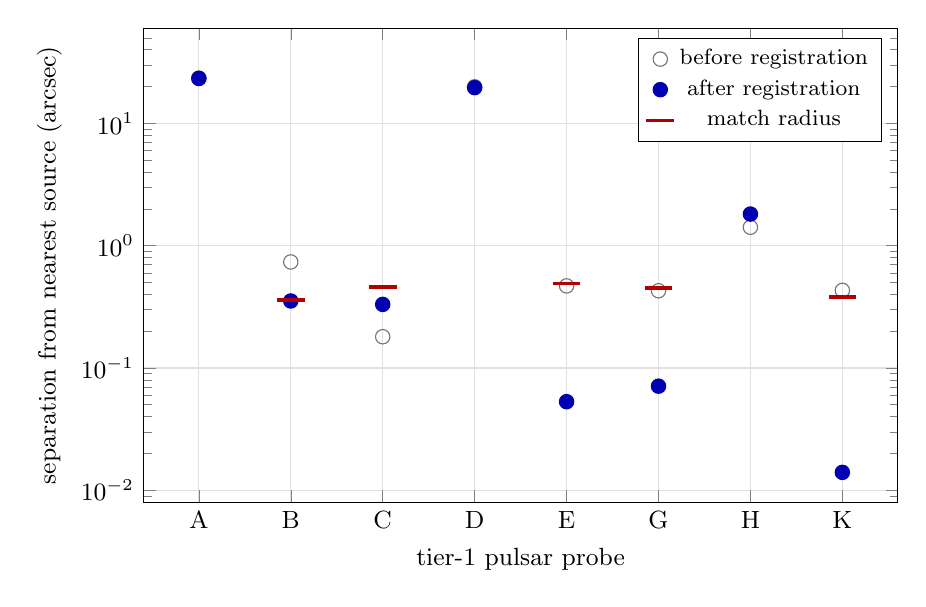
\begin{tikzpicture}
\begin{semilogyaxis}[
  width=0.92\linewidth, height=7.6cm,
  xlabel={tier-1 pulsar probe}, ylabel={separation from nearest source (arcsec)},
  xtick={1,2,3,4,5,6,7,8},
  xticklabels={A,B,C,D,E,G,H,K},
  xmin=0.4, xmax=8.6, ymin=0.008, ymax=60,
  legend style={font=\footnotesize, at={(0.98,0.98)}, anchor=north east},
  grid=major, grid style={black!12},
  tick label style={font=\small}, label style={font=\small},
]
\addplot[only marks, mark=o, mark size=2.6pt, black!55] coordinates {(1,23.468) (2,0.736) (3,0.180) (4,19.915) (5,0.469) (6,0.428) (7,1.415) (8,0.431)};
\addlegendentry{before registration}
\addplot[only marks, mark=*, mark size=2.6pt, blue!70!black] coordinates {(1,23.309) (2,0.353) (3,0.331) (4,19.596) (5,0.053) (6,0.071) (7,1.814) (8,0.014)};
\addlegendentry{after registration}
\addplot[only marks, mark=-, mark size=5pt, red!70!black, very thick] coordinates {(2,0.36) (3,0.46) (5,0.49) (6,0.45) (8,0.38)};
\addlegendentry{match radius}
\end{semilogyaxis}
\end{tikzpicture}
\caption{Tier-1 separations before and after the $(-0.081\as, +0.411\as)$ frame registration, with the match radius of each registered association marked. Registration moves B, E, G and K below their radii and moves H further away. A and D have no catalogue source within $19\as$ under either frame. Values from \texttt{analysis/results\_omega\_cen.json}.}
\label{fig:separations}
\end{figure}

\subsection{The MSP H association is discrepant}
\label{sec:results-h}

\citet{ZhaoHeinke2023} quote an offset of $0.73\as$ between MSP~H and their X-ray source h1, and cross-reference h1 to \citet{Henleywillis2018} source 14c. The timing position of \citet{ColomiBernadich2026} sits $1.415\as$ from the catalogue position of 14c, and $1.814\as$ from it after frame registration. The deviation runs in the opposite declination sense to the other five anchors, $-1.398\as$ against a $+0.42\as$ median.

Two explanations are available and we do not choose between them. Either 14c is not the \citet{Henleywillis2018} counterpart of source h1, in which case the cross-reference between the two catalogues is wrong for this row while both positions may be correct, or one of the two published positions is in error. Both are checkable, and the check is specific: the \citet{ZhaoHeinke2023} source list needs comparing against the \citet{Henleywillis2018} catalogue position by position. We have not done that, and it is not a question the vendored tables settle on their own.

The consequence for this paper is bounded. The primary frame registration (Section~\ref{sec:results-frame}) already excludes H; including it as a sensitivity check moves both medians by $\leq0.011\as$, well inside the six-anchor MAD of $0.103\as$/$0.161\as$, and changes no registered separation or match status at the $0.015\as$ precision quoted elsewhere in this paper. The discrepancy matters as a data-quality finding about the counterpart chain rather than because it moves any number here.

\subsection{Classification census}
\label{sec:results-class}

Published classes are taken verbatim from \citet{Henleywillis2018} and are not re-derived; the parenthesis convention of that catalogue marks non-members. The parse reproduces the paper's own abstract composition (Table~\ref{tab:classes}): 18 cataclysmic variables and candidates, one quiescent low-mass X-ray binary, four member variable stars, five anomalous-RGB or sub-subgiant stars, and one CH star, against 45 identifications in total.

\begin{table}[tbp]
\centering
\small
\caption{Published class census over all 233 catalogue sources \citep{Henleywillis2018}, membership as published. Source 24f is counted here under its published class (Section~\ref{sec:data-24f}).}
\label{tab:classes}
\begin{tabular}{llc}
\toprule
Class & Published membership & $n$ \\
\midrule
unidentified & no published statement & 188 \\
CV / CV candidate & member & 18 \\
AGN / AGN candidate & non-member & 9 \\
anomalous RGB / sub-subgiant & member & 5 \\
variable star & member & 4 \\
variable star & non-member & 4 \\
foreground star & non-member & 3 \\
quiescent LMXB & member & 1 \\
CH star (symbiotic candidate) & member & 1 \\
\bottomrule
\end{tabular}
\end{table}

Membership probabilities under the external normalisations of Section~\ref{sec:method-membership} are given in Table~\ref{tab:membership} and plotted in Figure~\ref{fig:membership}. The spread across assumptions is the result. Summed membership over the aperture runs from 53.1 to 86.0 sources as the assumed member count moves from 40 to 80 and the flux limit moves between its two settings, and the number of individual sources crossing $P_{\mathrm{member}} > 0.5$ runs from 0 to 67 over the same range. A binary membership label extracted from any single row of that table would be an artifact of the normalisation chosen.

\begin{table}[tbp]
\centering
\small
\caption{Membership sensitivity. Rows are the six combinations of assumed cluster-member count and background flux limit. Sums run over the 200 sources inside the $480\as$ aperture.}
\label{tab:membership}
\begin{tabular}{llccc}
\toprule
Assumed members & Flux limit & $N(P_{\mathrm{member}}>0.5)$ & $\sum P_{\mathrm{member}}$ & $\sum P_{\mathrm{member}}$ (unidentified) \\
\midrule
40 & core limiting  & 0  & 53.1 & 41.2 \\
40 & 5th percentile & 6  & 55.9 & 43.3 \\
60 & core limiting  & 27 & 69.5 & 54.0 \\
60 & 5th percentile & 38 & 72.7 & 56.5 \\
80 & core limiting  & 55 & 82.5 & 64.3 \\
80 & 5th percentile & 67 & 86.0 & 67.0 \\
\bottomrule
\end{tabular}
\end{table}

\begin{figure}[tbp]
\centering
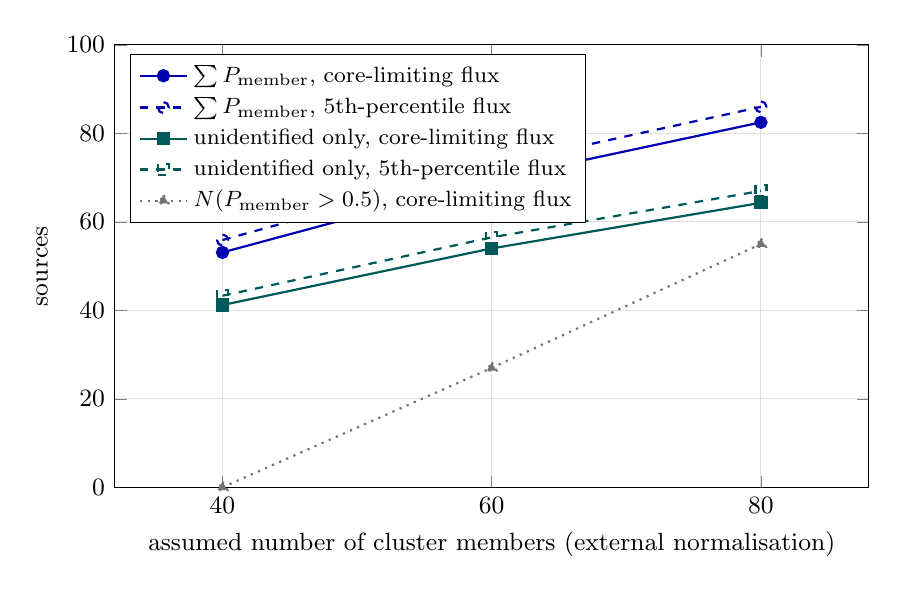
\begin{tikzpicture}
\begin{axis}[
  width=0.92\linewidth, height=7.2cm,
  xlabel={assumed number of cluster members (external normalisation)},
  ylabel={sources},
  xtick={40,60,80}, xmin=32, xmax=88, ymin=0, ymax=100,
  legend style={font=\footnotesize, at={(0.02,0.98)}, anchor=north west, cells={anchor=west}},
  grid=major, grid style={black!12},
  tick label style={font=\small}, label style={font=\small},
]
\addplot[blue!70!black, thick, mark=*] coordinates {(40,53.1) (60,69.5) (80,82.5)};
\addlegendentry{$\sum P_{\mathrm{member}}$, core-limiting flux}
\addplot[blue!70!black, thick, dashed, mark=o] coordinates {(40,55.9) (60,72.7) (80,86.0)};
\addlegendentry{$\sum P_{\mathrm{member}}$, 5th-percentile flux}
\addplot[teal!70!black, thick, mark=square*] coordinates {(40,41.2) (60,54.0) (80,64.3)};
\addlegendentry{unidentified only, core-limiting flux}
\addplot[teal!70!black, thick, dashed, mark=square] coordinates {(40,43.3) (60,56.5) (80,67.0)};
\addlegendentry{unidentified only, 5th-percentile flux}
\addplot[black!55, thick, dotted, mark=triangle*] coordinates {(40,0) (60,27) (80,55)};
\addlegendentry{$N(P_{\mathrm{member}}>0.5)$, core-limiting flux}
\end{axis}
\end{tikzpicture}
\caption{Membership ladder. Summed membership probability over the $480\as$ aperture, and over its unidentified subset, against the assumed external member normalisation at two background flux limits. The count of sources individually exceeding $P_{\mathrm{member}} = 0.5$ (dotted) moves from 0 to 55 over the same range, which is why membership is reported as a summed probability under stated assumptions and not as a label. Values from \texttt{analysis/results\_omega\_cen.json}.}
\label{fig:membership}
\end{figure}

\subsection{Background accounting}
\label{sec:results-agn}

Table~\ref{tab:agn} gives the expected background over the $0.05585\,\mathrm{deg^{2}}$ aperture at four candidate flux limits. The limit adopted for the residual is the fifth-percentile soft flux of the catalogue itself, $1.4\times10^{-16}\,\mathrm{erg\,cm^{-2}\,s^{-1}}$, giving 146.9 expected background sources with a bracket of 92.4 to 215.5. The core limiting flux scaled to the soft band gives a nearly identical 157.9, and the two lie well inside each other's brackets. The faintest tabulated flux lies below the fitted range of the \citet{Moretti2003} relation and is shown only to mark where extrapolation begins.

\begin{table}[tbp]
\centering
\small
\caption{Expected extragalactic background over the $480\as$ aperture at four candidate flux limits, from \citet{Moretti2003}. Brackets from the published parameter uncertainties used as symmetric widths. The row marked $\dagger$ lies below the relation's fitted flux range.}
\label{tab:agn}
\begin{tabular}{lcccc}
\toprule
Flux limit & $S$ ($\mathrm{erg\,cm^{-2}\,s^{-1}}$) & $N$ per $\mathrm{deg^{2}}$ & Expected in field & Bracket \\
\midrule
core limiting, scaled to soft & $1.24\times10^{-16}$ & 2827  & 157.9 & 99.0--232.5 \\
faintest tabulated soft$^{\dagger}$ & $1.00\times10^{-17}$ & 12852 & 717.8 & 417.2--1140.5 \\
fifth percentile soft (adopted) & $1.40\times10^{-16}$ & 2630  & 146.9 & 92.4--215.5 \\
median soft & $9.90\times10^{-16}$ & 787   & 43.9  & 29.4--60.7 \\
\bottomrule
\end{tabular}
\end{table}

\subsection{The residual census}
\label{sec:results-residual}

Inside the $480\as$ aperture the catalogue holds 200 sources, of which 41 carry a published identification (27 published members, 14 published non-members) and 159 do not. Eleven sources are confirmed MSP X-ray counterparts. Subtracting the adopted background expectation from the unidentified count gives
\begin{equation}
N_{\mathrm{residual}} = 159 - 146.9\,(92.4\text{--}215.5) = 12.1\ (-56.5,\ +66.6).
\end{equation}

The residual is background-dominated. Its central value is 8\,per~cent of the quantity subtracted and its bracket spans zero by a wide margin on both sides. The conservative reading is that the unidentified population inside this aperture is consistent with the extragalactic background alone, and that no excess is required by these data at this flux limit. Nothing in the rest of this paper should be read as claiming otherwise. What the residual does supply is a scale: an identification programme working through this field is working against a background that supplies of order 150 sources, and any cluster population it hopes to extract is a minority of the unidentified list.

Three accounting conventions change the number and are stated here. Published non-member AGN identifications sit in the identified column, so the subtraction removes a predicted background from a population that already excludes background sources someone has taken the trouble to identify, which biases the residual low. The aperture excludes 33 catalogue sources from both sides, so this is not a statement about the full 233. And the eleven confirmed MSP X-ray counterparts are retained in the unidentified column, since the catalogue's own optical-identification field predates the pulsar timing set; removing them would lower the residual by that count, well inside the quoted bracket.

\subsection{The MSP-like region}
\label{sec:results-msplike}

The confirmed counterparts define a region in the colour-flux plane from this cluster's own data. Four of them ($n=4$: 23g, 11f, 24f, 21d) carry both a tabulated colour and a flux and anchor it; a fifth recovered counterpart lacks a tabulated colour and is dropped. The primary construction is a bounding box on those same four anchors: counting unidentified sources inside it gives 39, of which 14.85 survive membership weighting at the adopted normalisation. A $2\sigma$ ellipse on the same $n=4$ anchors, reported as a secondary and wider construction, gives 53 (19.44 weighted). Eleven unidentified sources carry neither a colour nor a flux and cannot be placed in the plane at all. Neither region screens for background AGN, so the 39 and 53 counts are upper bounds on MSP-like membership rather than membership estimates.

This is not the ``more than 30 MSP-like'' count of \citet{Henleywillis2018}. That criterion compares against MSPs in other clusters and is not tabulated in the source paper, so it cannot be reproduced from the machine-readable table. The region used here is defined from four counterparts in this cluster, a different construction with a different systematic. The two numbers are not interchangeable, and the numerical proximity of 39 to ``more than 30'' is a coincidence of construction rather than a confirmation.

\section{The population disagreement}
\label{sec:tension}

Two published estimates of the total pulsar population of \ocen{} are available and they disagree by a factor of 54. \citet{Yin2024} report an empirical-Bayesian escape-velocity scaling relation that predicts 324 pulsars at this cluster's escape velocity of $62.2\,\mathrm{km\,s^{-1}}$. The encounter-rate estimate they tabulate alongside it gives 6.

Against 19 known pulsars those totals imply 305 and 0 undiscovered. The X-ray detection fraction measured in this cluster depends on which denominator is used: \citet{ZhaoHeinke2023} found 11 counterparts among the 18 MSPs known and searched at the time of their work (0.611), while 19 pulsars are known today and the 19th was never searched, not a non-detection, so the conservative variant against today's full count is 11 of 19 (0.579). We carry both rather than choosing: applying 0.611 gives 186.4 and applying 0.579 gives 176.6 X-ray-detectable undiscovered pulsars from the escape-velocity model; the encounter-rate model gives 0.0 under either fraction, since it predicts zero undiscovered pulsars (Table~\ref{tab:pop}).

\begin{table}[tbp]
\centering
\small
\caption{Population predictions from \citet{Yin2024}, carried as a bracket. The final two columns apply the X-ray detection fraction measured in this cluster under its two denominators: 0.611 (11 of the 18 MSPs \citet{ZhaoHeinke2023} searched) and 0.579 (11 of the 19 known today, conservative).}
\label{tab:pop}
\begin{tabular}{lcccc}
\toprule
Model & Predicted total & Undiscovered & X-ray-detectable (0.611) & X-ray-detectable (0.579) \\
\midrule
escape velocity & 324 & 305 & 186.4 & 176.6 \\
encounter rate  & 6   & 0   & 0.0   & 0.0 \\
\bottomrule
\end{tabular}
\end{table}

The escape-velocity number exceeds the residual of 12.1 by more than an order of magnitude, and exceeds the full unidentified count of 159 once the background is not subtracted. That bounds the extrapolation, the assumed detection fraction, or the background subtraction, and this analysis does not decide which. Three reasons keep each candidate live.

\textbf{The extrapolation.} The \citet{Yin2024} relation was fitted on FAST-visible clusters. \ocen{} at $\delta = -47^{\circ}$ is not FAST-visible, so applying the relation here reaches outside the sample it was fitted on, in a cluster whose escape velocity places it at the top of the predicted range.

\textbf{The detection fraction.} The measured 0.611 (or 0.579 against today's full known count) is the fraction of searched pulsars with a Chandra counterpart. Applying it to the undiscovered population assumes those pulsars share the X-ray luminosity distribution of the discovered ones. Radio-faint or large-radius pulsars need not, and the discovered set is selected in ways that correlate with X-ray brightness, so either fraction is more plausibly an upper bound than an unbiased estimate.

\textbf{The background subtraction.} Eddington bias inflates the faint fluxes on which the background limit is computed, which makes the expected background a lower bound and the residual an upper bound. Correcting the residual downward would widen the gap rather than close it.

Adjudicating it requires the identification work this census is meant to enable, not a preference asserted here.

\section{Discussion}
\label{sec:discussion}

\subsection{What would identify the residual}
\label{sec:disc-future}

The residual is an input to identification work, and the useful output of this paper is a specific list of what that work requires. Each item below is a concrete, currently blocked step, ordered by cost.

\textbf{The six missing pulsar positions.} F, J, M, O, P and R carry no position in \citet{ColomiBernadich2026}. Recovering them from \citet{Chen2023} would extend the probe set by six probes and is the cheapest available improvement to every number in Section~\ref{sec:results}.

\textbf{The counterpart-chain check.} The MSP~H discrepancy of Section~\ref{sec:results-h} is resolvable by comparing the \citet{ZhaoHeinke2023} source list against the \citet{Henleywillis2018} catalogue position by position. It requires no new observation.

\textbf{Exposure-map membership.} The degeneracy of Section~\ref{sec:method-membership} is instrumental and is fixed by the Chandra exposure map, which turns a spatial fit that cannot separate the cluster profile from the sensitivity profile into one that can. Membership would then be fitted rather than normalised externally, and the six-row sensitivity table of Table~\ref{tab:membership} would collapse to one row with an error bar.

\textbf{Variability with epoch-resolved data.} No variability analysis appears in this paper. Both the 2000 and 2012 Chandra epochs exist and the catalogue tabulates a flux ratio between them, but a single ratio does not support a statistically valid variability test at these count rates, and epoch-resolved event data are not staged here. This is the clearest gap between what this paper does and what a full identification programme needs, since variability is what separates quiescent binaries from background AGN when colour does not.

\textbf{Deeper radio positions.} Sub-arcsecond positions for the tier-2 pulsars would move five probes out of a tier whose uncertainty rule is a convention of ours rather than a measurement.

\subsection{The census as an anomaly screen}
\label{sec:disc-anomaly}

A complete accounting of a cluster's X-ray sources doubles as a screen for sources fitting no known class, a standard byproduct of catalogue work worth one sentence of acknowledgement in a series that elsewhere considers non-astrophysical hypotheses \citep{Swanson2026Engineered}. This census does not perform that screen. The residual computed here is background-dominated, consistent with zero, and defined by the absence of an optical identification rather than by any positive property; treating it as a population of anomalies would require the identification work Section~\ref{sec:disc-future} lists as outstanding, and until that work is done the residual carries no information about the nature of its members.

\section{Conclusion}
\label{sec:conclusion}

We have cross-matched the 233-source Chandra catalogue of \citet{Henleywillis2018} against the 19-pulsar timing set of \citet{ColomiBernadich2026}, validated the pipeline on 47~Tucanae first, and reported what is left.

The control recovers 18 of 21 known counterparts at the 95\,per~cent match radius and misses the three rows the control catalogue itself flags. The \ocen{} Chandra frame carries a measured $+0.41\as$ declination offset against the radio frame; registering it takes tier-1 matches from three of eight to five of eight, and the five registered associations sit between $0.01\as$ and $0.35\as$ with chance-coincidence probabilities below $2.3\times10^{-3}$ under three independent estimators. The published association of MSP~H with source 14c does not survive registration, sitting at $1.81\as$ in the wrong declination sense, which we record as a data-quality finding requiring a position-by-position check of the counterpart chain.

The residual census inside a $480\as$ aperture is 12.1 unidentified sources $(-56.5, +66.6)$ after subtracting a background expectation of 146.9 (92.4--215.5), which is to say it is consistent with the background alone. Between 39 and 53 unidentified sources fall in a colour-flux region defined by this cluster's own confirmed counterparts, a quantity constructed differently from the catalogue's own ``more than 30'' and not interchangeable with it. The two published population predictions differ by a factor of 54, and the larger over-predicts the residual by more than an order of magnitude, which bounds the extrapolation, the detection fraction, or the background subtraction without deciding among them.

\section*{Data availability}

The analysis pipeline (\texttt{crossmatch.py}, \texttt{classify.py}, \texttt{residual.py}, \texttt{run\_g.py}), its fixed seed, its two results files and the mechanical analysis report accompany this paper under \texttt{paper/g/analysis/}. The vendored source catalogues, their checksums and their provenance record are under \texttt{paper/g/data/}. Both source catalogues are public at VizieR (\texttt{J/MNRAS/479/2834} and \texttt{J/MNRAS/472/3706}).

\appendix

\section{Caveat checklist}
\label{app:caveats}

The following are stated as limitations of this analysis and are not corrected for.

\begin{enumerate}
\item \textbf{Eddington bias.} Fluxes near the detection limit are biased high, so a background count computed above a limit derived from those same fluxes is a lower bound on contamination. No deboosting is possible without the detection-significance distribution, which the vendored table does not carry.
\item \textbf{Completeness varies with off-axis angle} across the ACIS-I field. A single flux limit is applied over the whole area, which overestimates the effective depth at large radius and therefore overestimates the background count there while underestimating the true source count.
\item \textbf{No variability analysis} is performed. Epoch-resolved data are not staged and the single tabulated 2012/2000 flux ratio does not support a Poisson-honest test. Explicitly out of scope, and the largest departure from what a full identification programme requires.
\item \textbf{The residual is an input to future identification work.} It is not a detection and it is not evidence for any hypothesis.
\item \textbf{Chance-coincidence rates} are reported per probe by three independent estimators and are never collapsed into one number.
\item \textbf{Membership} is reported as a probability under stated external normalisations, never as a binary label, and every published membership statement is carried alongside rather than overwritten.
\item \textbf{The tier-2 positional uncertainty rule} is a convention of this analysis (one unit in the last quoted digit), not a value stated by the source paper.
\item \textbf{The escape-velocity population relation} was fitted on FAST-visible clusters and \ocen{} is not FAST-visible, so its prediction here is an extrapolation.
\item \textbf{The background-relation parameter uncertainties} are published asymmetrically and are used here only as symmetric bracket widths; no asymmetric error is quoted.
\item \textbf{The internal membership fit is degenerate} and is reported as a diagnostic only; membership uses external normalisations throughout.
\item \textbf{The control is an optimistic bound.} The control catalogue was itself astrometrically registered against its MSP truth set, so control recovery bounds match performance from above rather than testing astrometry independently.
\item \textbf{Six pulsars are absent} from the cross-match for want of a published position, so every match count is conditional on a 13-probe subset of the 19-pulsar timing set.
\end{enumerate}

\bibliographystyle{apalike}
\bibliography{../references,../engineered-extra,census-extra}

\end{document}
